\chapter{Demonstration of Baseline Compensation System} \label{chap5}
In this chapter, the demonstration of the baseline compensation system is described. The purpose of this demonstration is to compensate for the deformation of the baseline so that the length fluctuation of the 3-km arm cavity is reduced below 1 Hz, where the passive seismic isolation cannot attenuate the seismic disturbance. 

In the section \cref{sec:sec51}, experimental arrangement for demonstration is described. In section \cref{sec:sec52}, the result of the test is described. In the end, the discussion is described in section \cref{sec:sec53}.

\section{Experimental Arrangement} \label{sec:sec51}
Because the purpose of the baseline compensation system is to reduce the arm cavity length fluctuation, we prepared the experimental arrangement to measure the length.

\subsection{Measurement of X-arm cavity length}
The length fluctuation of the X-arm cavity is measured by the PDH method \cite{drever1983laser}. This method obtains the error signal, which is proportional to the displacement from the nominal length where the cavity is on resonance. In order to keep the resonance, the error signal is fed back to the acousto-optics modulator (AOM), which changes the input laser frequency.

Brief measurement procedure is shown in Figure \ref{img:img600}. (1) The deformation of the baseline causes the length change of the arm cavity length through the suspensions. Suppose that the baseline length is displaced by $\Delta{L}$ from the nominal length
of $L$. Utilizing the PDH method, we can obtain the error signal proportional to this displacement. (2) This signal is also interpreted as the frequency changes of the input laser because the frequency change $\Delta{f}$ has a relation with the baseline length change $\Delta{L}$ \cite{izumi2012multi};
\begin{eqnarray}
  \displaystyle -\frac{\Delta{f}}{f} = \frac{\Delta{L}}{L}.
\end{eqnarray}
(3) To keep the optical cavity on resonance, the signal is fed back to the AOM, which is the frequency actuator. In this procedure, the length fluctuation is obtained from the feedback signal to the AOM.
\begin{figure}[h]
  \centering
  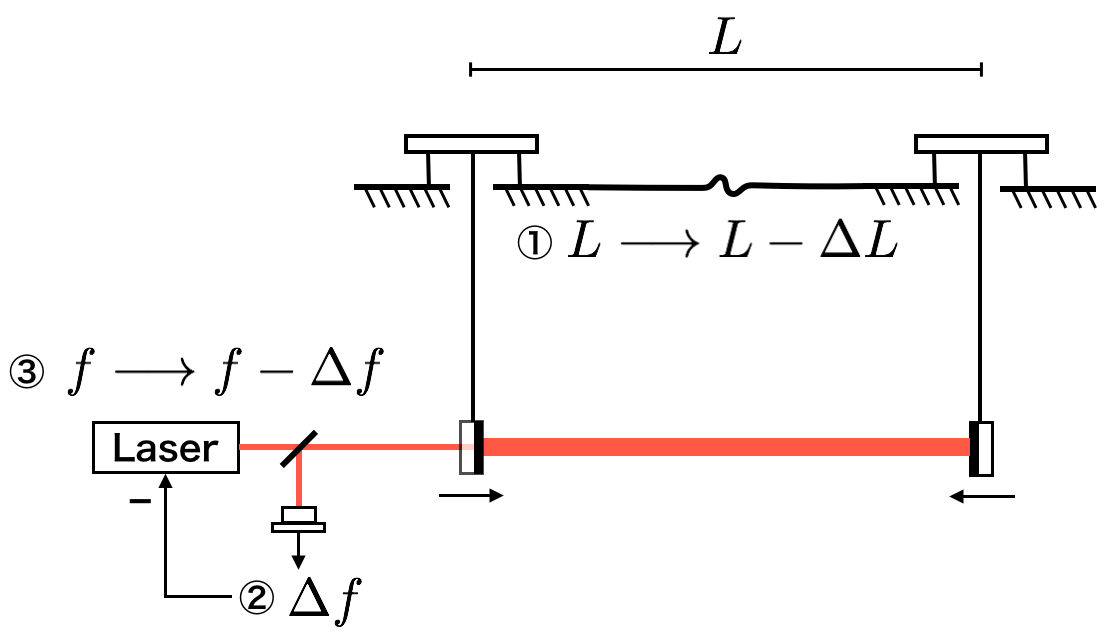
\includegraphics[width=13cm]{./img_chap6/img600.png}
  \caption{Experimental arrangement for X-arm length measurement. X-arm cavity controled by feeding the PDH signal back to the AOM of the input laser to keep on resonance. The length change of the cavity is obtained from the feedback signal.}
  \label{img:img600}  
\end{figure}



\subsection{Control Design}
\begin{figure}[h]
  \begin{minipage}{14cm}
    \begin{center}   
      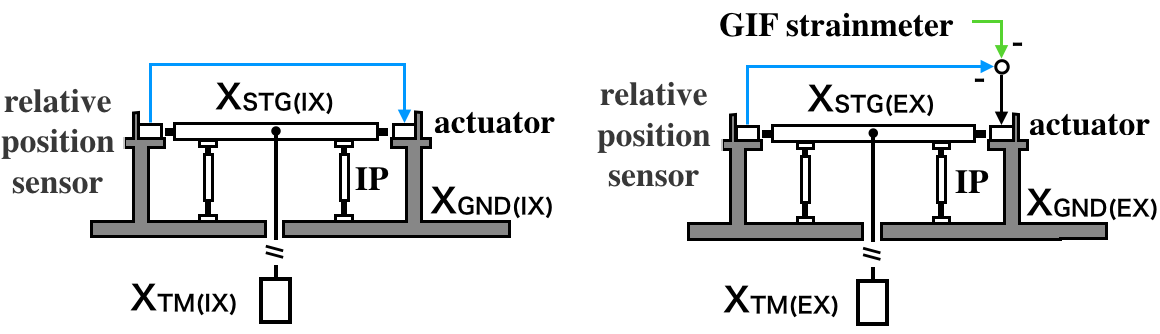
\includegraphics[width=14cm]{./img_chap6/img630a.png}
      \subcaption{Schematic contol of each platform stage. Left figure is that of the IX stage, right figure is that of the EX.}\label{img:img630a} \hfill\vspace{10pt}
    \end{center}
  \end{minipage}
  \begin{minipage}{14cm}
    \begin{center}   
      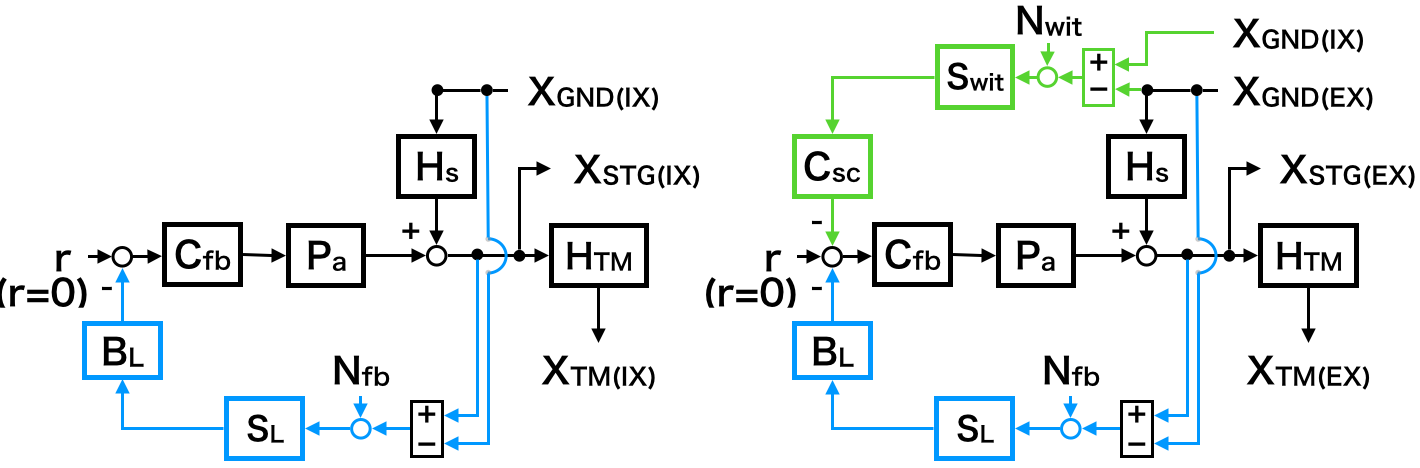
\includegraphics[width=14cm]{./img_chap6/img630b.png}
      \subcaption{Control block diagram of each platform stage. Left figure is that of the IX stage, right figure is that of the EX.}\label{img:img630b}
    \end{center}
  \end{minipage}
  \caption{The baseline compensation control of each platform stage for demonstration.}
\end{figure}

To demonstrate the baseline compensation system using GIF, we design a simple control configuration. Although the simplest configuration is the feedforward using the GIF, the feedforward control cannot suppress the disturbances other than the horizontal seismic noise such as the tilt ground motion or the temperature fluctuation \cite{sekiguchi2016astudy}. Because these disturbances could move the platform stage in a horizontal direction, we need a feedback control using the position sensor to suppress these disturbances. Therefore we use the sensor correction control rather than the feedforward control. 

Figure \ref{img:img630a} shows the schematic control of the platform stage for the input x-arm test mass (IX) and end x-arm test mass (EX). While the IX stage is fed back the relative position sensor signal to the actuator on the stage, the EX stage is added to the GIF strainmeter signal. In other words, while the IX stage is locked to the local IX ground, the EX stage is also locked to the local EX ground, but this feedback signal is corrected by using the GIF strainmeter. The GIF measure the baseline length changes, which means the differential motion of the IX and EX ground. Therefore, the feedback signal corrected by using GIF is the same as the feedback signal of the IX stage. Thus, the EX stage can follow the IX stage by using the corrected feedback signal.

Figure \ref{img:img630b} shows the control diagram of each stage. In both stages, the displacement of the IX platform stage $X_{\mathrm{STG}}$ is disturbed by the local seismic motion $X_{\mathrm{GND}}$ though the mechanical response of the inverted pendulum (IP) $H_{\mathrm{s}}$. Moreover, the displacement of the IX test mass is also disturbed by this seismic noise through the mechanical response of the pendulum $H_{\mathrm{TM}}$. In order to reduce the test mass motion in the low-frequency region, below 1 Hz, the platform stage is controlled by the feedback control using the relative position sensor. $S_{\mathrm{L}},\, N_{\mathrm{fb}}$ and $B_{\mathrm{L}}$ are the displacement response and the noise of the relative position sensor and the low-pass filter not to inject the sensor noise to the feedback signal. The feedback signal is sent to the actuator, whose transfer function from the actuator force to the platform stage is given by $P_{\mathrm{a}}$, through the control filter $C_{\mathrm{fb}}$. On the other hand, the feedback signal of the EX stage is corrected by the GIF signal.

In this situation, each displacement of the stage are given by 
\begin{eqnarray}
  X_{\mathrm{STG(IX)}} &=& \displaystyle\frac{G}{1+G} X_{\mathrm{GND(IX)}} + \frac{G}{1+G} N_{L} + \frac{1}{1+G} H_{\mathrm{s}} X_{\mathrm{GND(IX)}} \\ \nonumber,
  X_{\mathrm{STG(EX)}} &=& \displaystyle\frac{G}{1+G} \left(1- \frac{C_{\mathrm{sc}}S_{\mathrm{wit}}}{B_{\mathrm{L}}S_{\mathrm{L}}}\right) X_{\mathrm{GND(EX)}} + \frac{G}{1+G}N_{L} \\ \nonumber
  &+& \frac{G}{1+G} \frac{C_{\mathrm{sc}}S_{\mathrm{wit}}} {B_{\mathrm{L}}S_{\mathrm{L}}} X_{\mathrm{GND(IX)}}
  + \frac{G}{1+G} \frac{C_{\mathrm{sc}}S_{\mathrm{wit}}} {B_{\mathrm{L}}S_{\mathrm{L}}} N_{\mathrm{wit}}\\ 
  &+& \frac{1}{1+G} H_{\mathrm{s}} X_{\mathrm{GND(EX)}},
\end{eqnarray}
respectively, where $G=C_{\mathrm{fb}}P_{\mathrm{a}}S_{\mathrm{L}}B_{\mathrm{L}}$ is the loop gain. Here, if $G\gg1$ and we design the sensor correction filter $C_{\mathrm{sc}}$ so that
\begin{eqnarray}
  \frac{C_{\mathrm{sc}}S_{\mathrm{wit}}}{B_{\mathrm{L}}S_{\mathrm{L}}} = 1,
\end{eqnarray}
the displacement of each stage are give as 
\begin{eqnarray}
  X_{\mathrm{STG(IX)}} &=& X_{\mathrm{GND(IX)}} + N_{\mathrm{L}},\\
  X_{\mathrm{STG(EX)}} &=& X_{\mathrm{GND(IX)}} + N_{\mathrm{L}} + N_{\mathrm{wit}}.
\end{eqnarray}
Moreover, if the noise of the GIF, which is the wittness sensor is smaller than that of the relative position sensor, both stage motions are the same each other; $X_{\mathrm{STG(EX)}}=X_{\mathrm{STG(IX)}}$. This same motion means the reduction of the differential stage motion. Thus, the cavity length is isolated from the differential ground motion, which is the baseline length fluctuation.




\section{Results and Discussion } \label{sec:sec52}
The performance of the baseline compensation system is evaluated when the system is engaged.

\subsection{Results}
\begin{figure}[h]
  \centering
  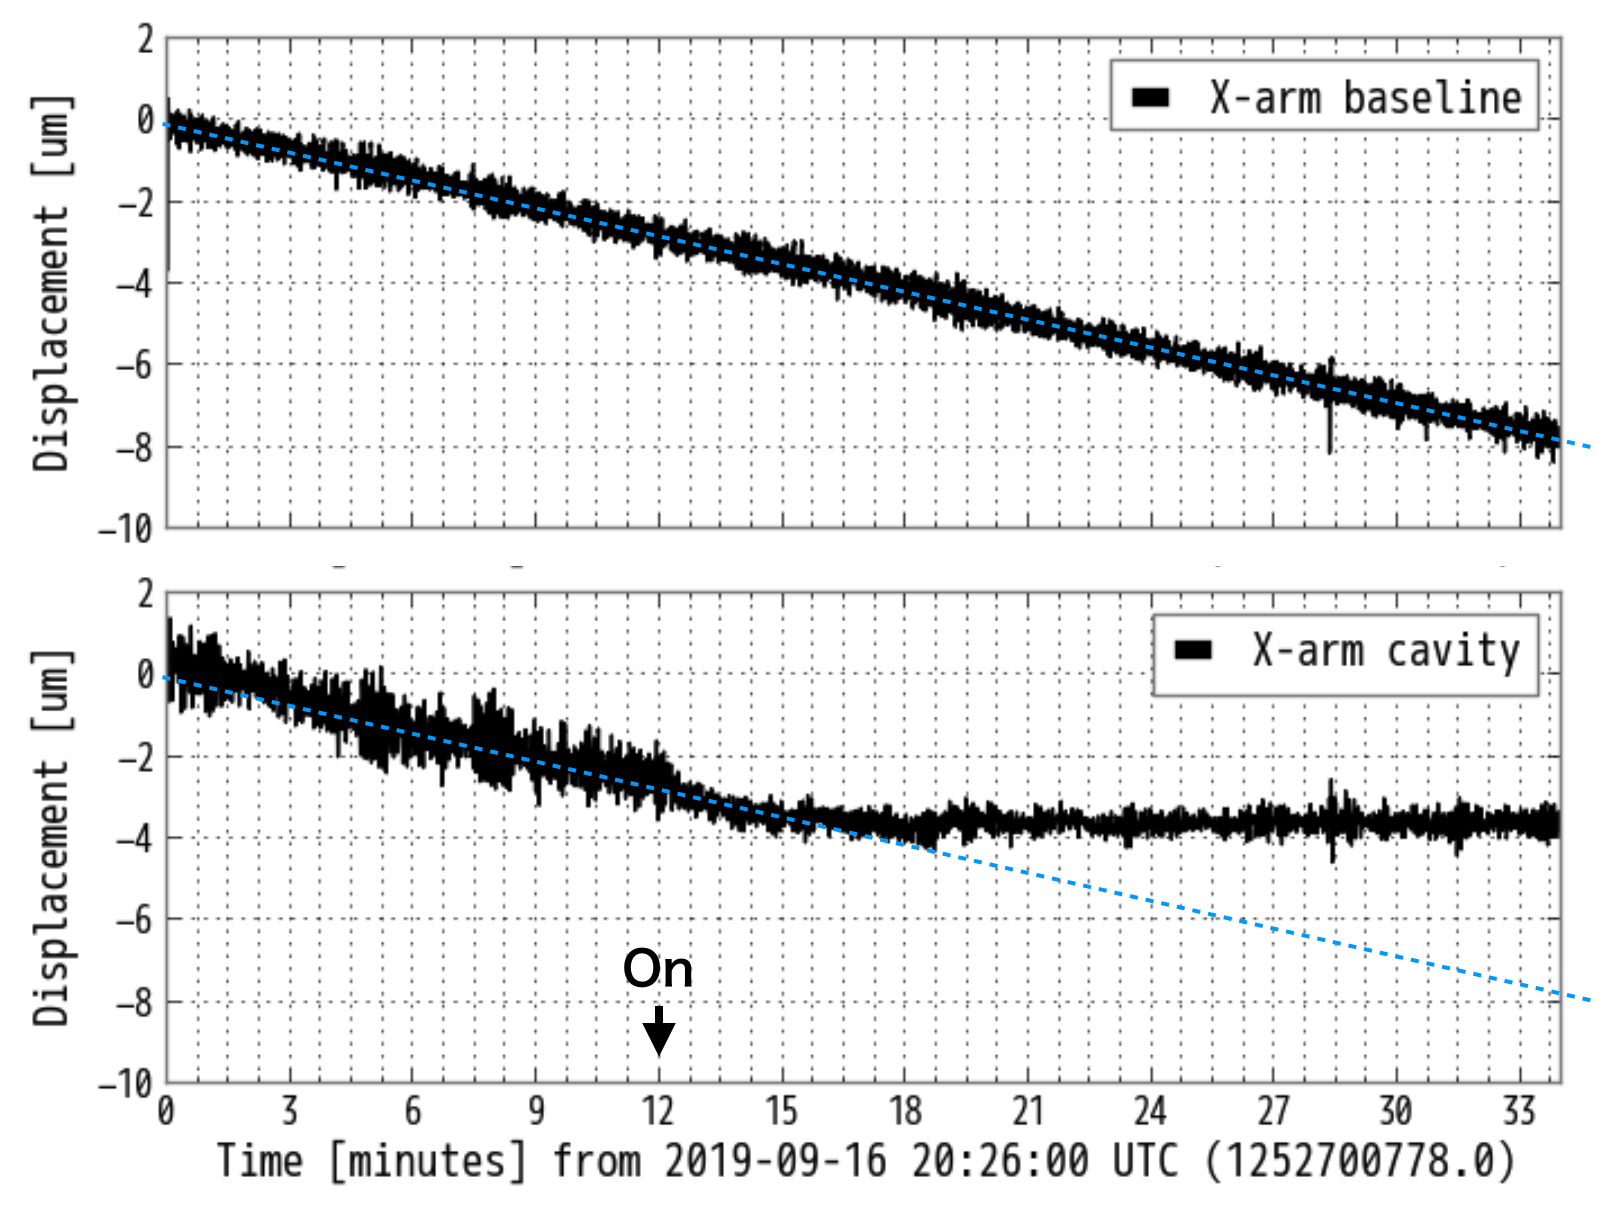
\includegraphics[width=12cm]{./img_chap6/img610.png}
  \caption{Length change of both X-arm baseline and X-arm cavity when baseline compensation system is turned on or off. At 12 minutes, the control is on.}\label{img:img610}
\end{figure}

Figure \ref{img:img610} shows the length fluctuation of the arm cavity and of the baseline as a reference. At 12 minutes, the baseline compensation system was turned on. Whereas the X-arm cavity length is drifted during the compensation system was off, the drift is removed during the system was on. This drift is comparable to the earth tide. As a result, this system compensated the deformation of the baseline, and the reduction ratio is almost 1/10.

This result also indicates that the RMS amplitude of the X-arm cavity length is reduced. The amplitude spectrum density of the length when both the compensation system was on and off is shown in Figure \ref{img:img611}. It is clear that the accumulated RMS amplitude is reduced due to the compensation system. In the next, we compare this measured data with the rigid body model.

\begin{figure}[h]
  \centering
  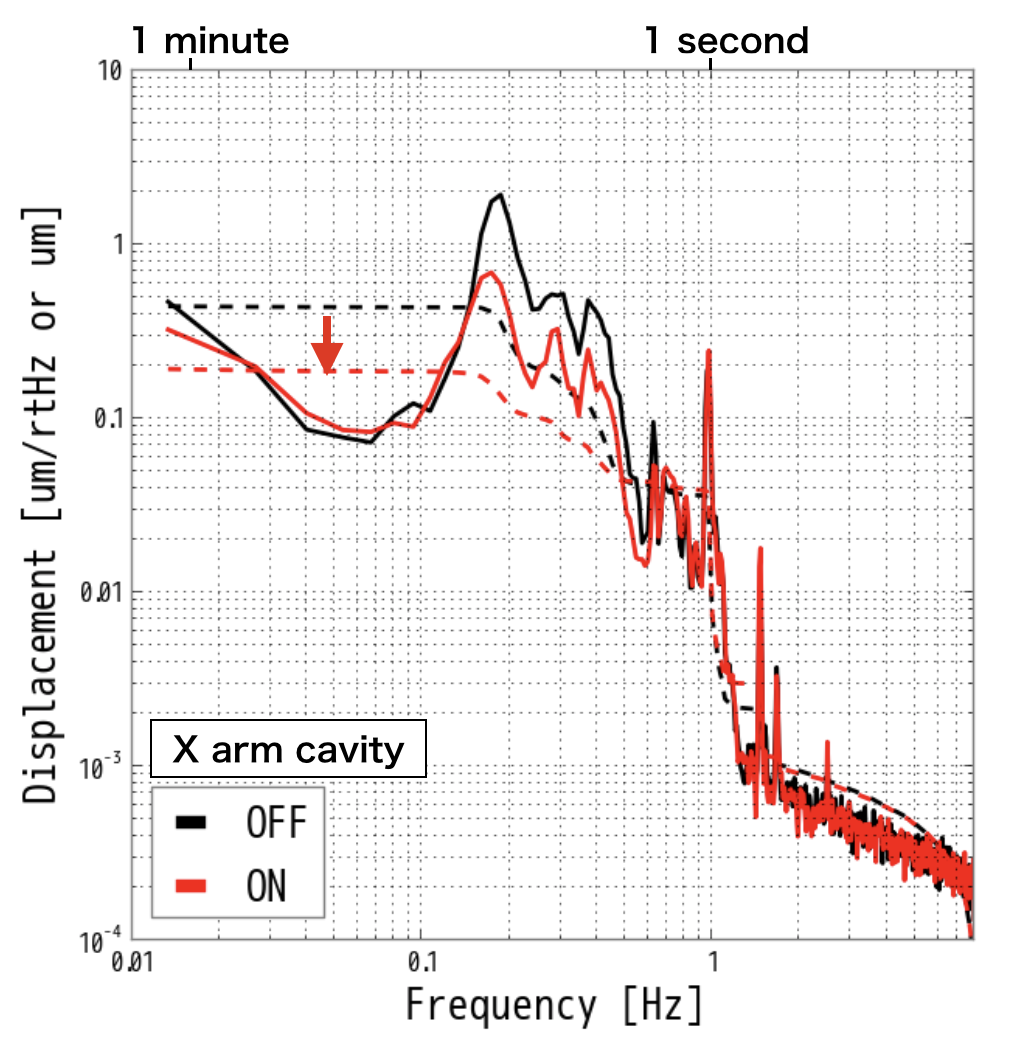
\includegraphics[width=10cm]{./img_chap6/img611.png}
  \caption{ASDs of X-arm caivty length when baseline compensation system is turned on and off. }\label{img:img611}
\end{figure}

\subsubsection{Comparison with the model}
Compare with the measured data and rigid body model of the KAGRA suspensions \cite{sekiguchi2016astudy}. Because this model outputs the state-space model, we can calculate the transfer function. For example, the transfer function from the ground motion to each stage; the platform stage, test mass, and so on.

To simplify the discussion, suppose the CMRR is large enough to ignore the coupling from the common motion to the differential motion, as described in \cref{sec532}. It is a valid assumption below the eigenfrequency of the suspensions. According to Eq.(\ref{eq:eq518}), the transfer function from the differential input to differential output is given by a single transfer function. Therefore, the differential transfer functions from the differential ground motion to the differential output of the stage and the test mass motion are given by the single transfer function of that, respectively.

\begin{figure}[p]
  \begin{minipage}{14cm}
    \centering
    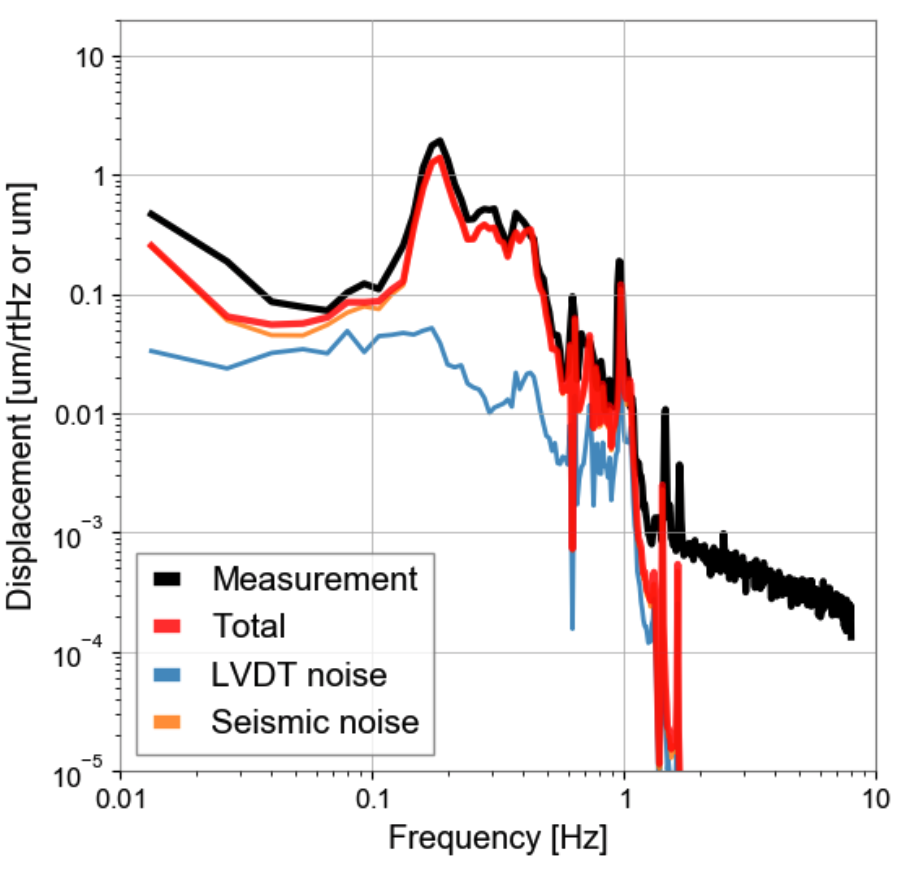
\includegraphics[width=9cm]{./img_chap6/img612.png}
    \subcaption{Noise budget when the compensation system is OFF. Measurement is same as the black line in Fig.\ref{img:img611}. Total is the summation of all the noise contributions.}\label{img:img612} %\hfill\vspace{5pt}
  \end{minipage} 
  \begin{minipage}{14cm}
    \centering
    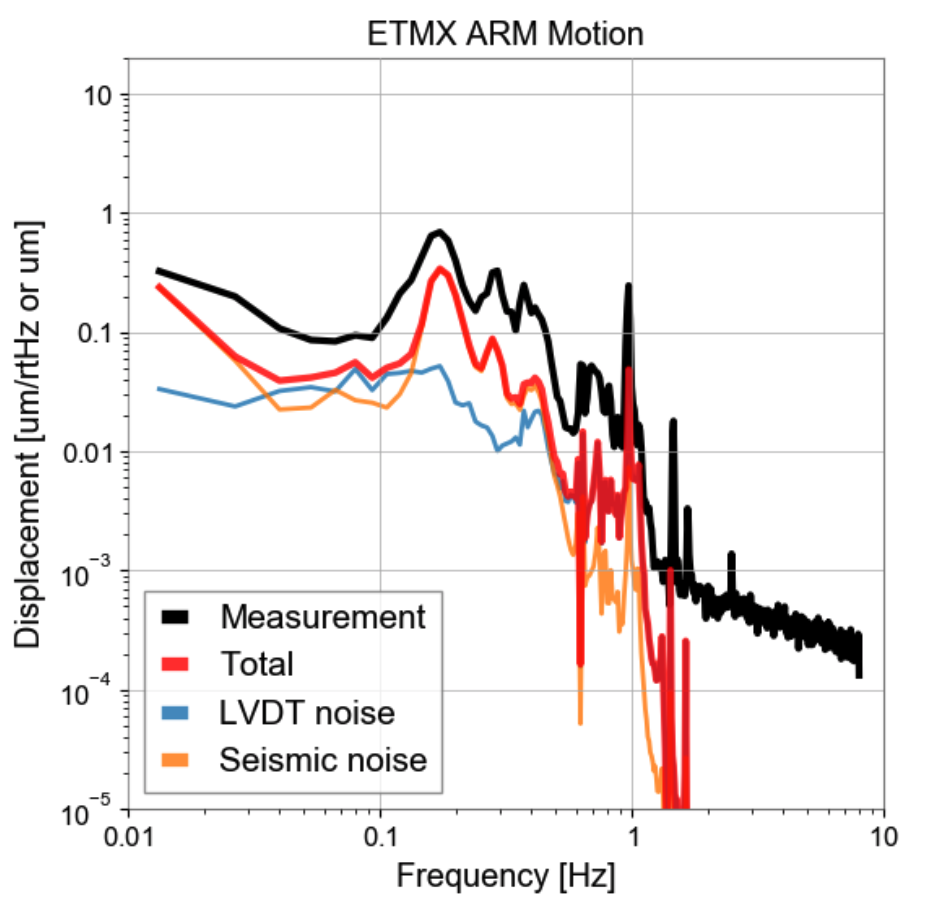
\includegraphics[width=9cm]{./img_chap6/img613.png}
    \subcaption{Noise budget when the compensation system is ON. Measurement is same as the red line in Fig.\ref{img:img611}. Total is the summation of all noise contributions assuming the reduction factor of sensor correction of 1/20.}\label{img:img613}
  \end{minipage}
  \caption{Comparison between the measurement of X-arm and expected value of that. The expected total value is the summation of some noise contribution, which is named noise budget. }
\end{figure}

Figure \ref{img:img612} shows the amplitude spectrum densities (ASDs) of the X-arm cavity length when the compensation system is OFF. The black line is the ASD calculated by the feedback signal of the X-arm cavity. The red line is the ASD, which is the summation of the noise contributions, the noise of the relative position sensor, named LVDT (blue line), and the noise of the differential baseline length change measured by the GIF strainmeter (orange line). Above 1 Hz, the X-arm cavity length and the seismic noise contribution are not the signals due to the noises of the instruments. Below 1 Hz, the measurement is consistent with the estimation.

Figure \ref{img:img613} shows the ASDs of the X-arm cavity length when the compensation system is ON. The red line, which indicates the summation of the noise contribution estimated by the rigid body model, is calculated assuming the reduction factor of the sensor correction of 1/20, as mentioned in \cref{sec:sec513}. This reduction factor is calculated from the relative calibration error of 5 \% between the LVDT and GIF. Although this reduction rate should be realized, the measurement is not consistent with the estimation assumed the reduction rate. The RMS of the cavity length fluctuation is limited by peaks around 200 mHz.

\subsection{Discussion}
The peaks around 200 mHz, which are the main contributions to the RMS, are correlated with the other degrees of freedoms (DOFs). 

Figure \ref{img:img614} shows the ASDs in the top figure and the coherence in the bottom figure when the compensation system was off. In the top figure, the ASDs of the X-arm cavity length and the baseline length changes are displayed. The baseline length changes are shown by two ASDs; the length change measured by the GIF strainmeter and that given by the differential signal of two seismometers, which is installed near the IX and EX stages. While, above 1 Hz, the baseline length change should be referred by the seismometer differential signal, below 50 mHz, the length change should be referred by the GIF strainmeter signal because of this self-noise. One can find that the X-arm cavity length is enhanced by some mechanical peaks compared with the baseline length change. On the other hand, the bottom figure shows some coherence between the X-arm cavity length and the GIF, and between the cavity length and the other DOFs' signals; the feedback signals of the yaw and transverse directions on the each IX and EX platform stages, which controls are needed to keep the X-arm cavity on resonance. Whereas the cavity length has a coherence with the deformation of the baseline measured by GIF strainmeter (blue) around 0.2 - 0.7 Hz broadly, coherence with the other DOFs does not exist clearly in this frequency region. This coherence implies that the cavity length is mainly disturbed by the deformation of the baseline.

Figure \ref{img:img615} show the ASDs and coherence when the compensation system was on. Around 0.2 Hz, the coherence between the cavity length and the many other DOFs appear, although these coherences did not when no length compensation. These coherences imply the cavity length is disturbed by the internal DOFs coupling.

\begin{figure}[p]
  %\begin{minipage}{14cm}
    \centering
    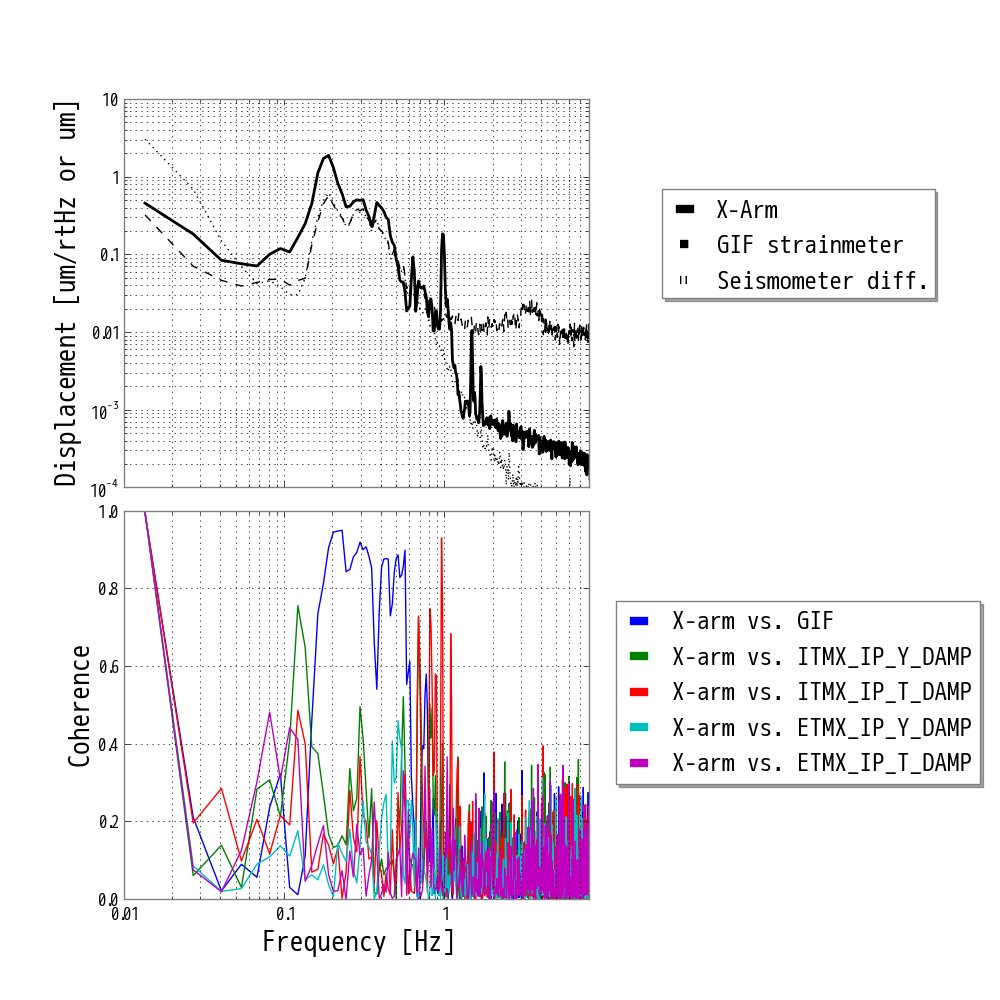
\includegraphics[width=15cm]{./img_chap6/img614.png}
    \caption{Coherence between the cavity length and GIF strainmeter, other degrees of freedoms on the stage control when the compensation system is on. (Top) ASD of the cavity length and baseline length. (Bottom) The coherence between the cavity's length and some signals.}\label{img:img614}
    %\end{minipage}
\end{figure}
\begin{figure}[p]
  %\begin{minipage}{14cm}
    \centering 
    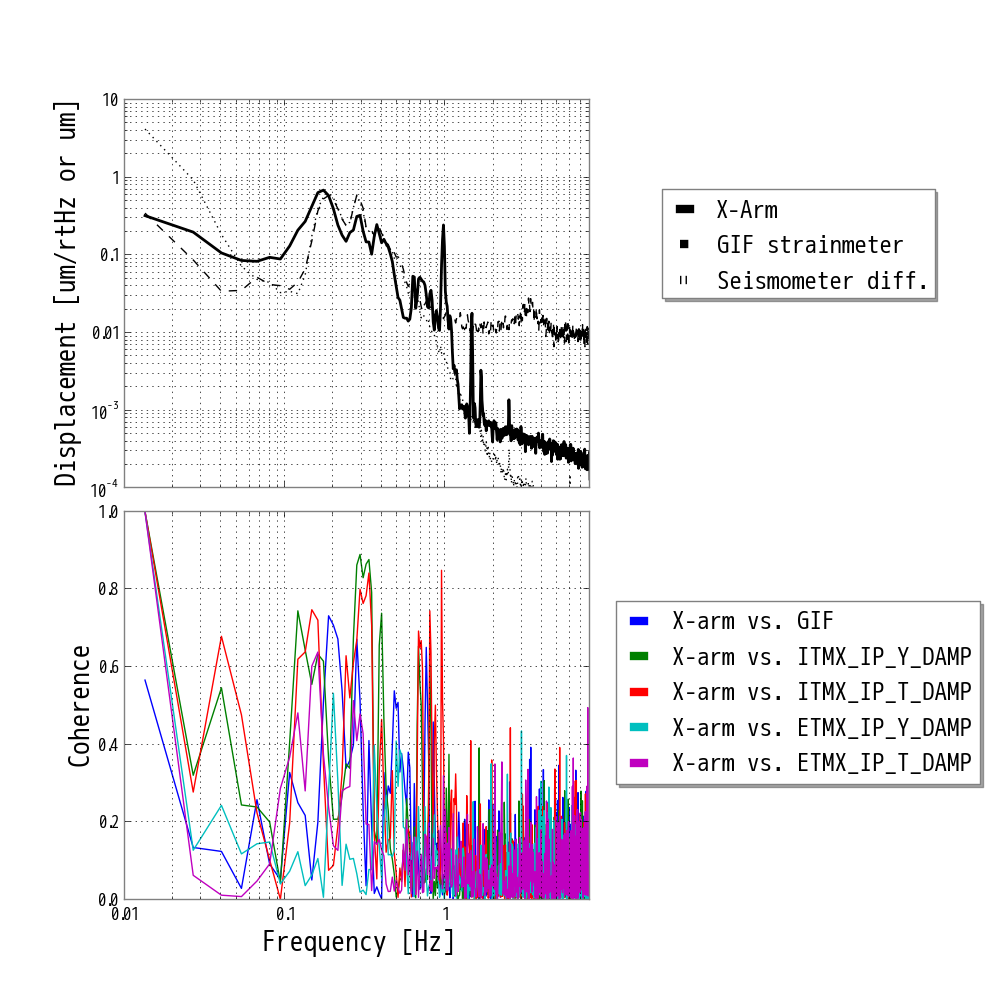
\includegraphics[width=15cm]{./img_chap6/img615.png}
    \caption{Coherence between the cavity length and GIF strainmeter, other degrees of freedoms on the stage control when the compensation system is off. (Top) ASD of the cavity length and baseline length. (Bottom) The coherence between the cavity's length and some signals.}\label{img:img615}
  %\end{minipage}  
\end{figure}



\section{Summary of the Chapter} \label{sec:sec53}
In this chapter, the following items are described:
\begin{itemize}
\item Experimental arrangement for evaluation of the X-cavity length fluctuation was described.
\item As a result, above 1 minutes period, the fluctuation is reduced by 20 dB, while below this period, the fluctuation is reduced by 6 dB.
\item According to the coherence measurement, the internal coupling to the cavity length would limit the performance in the short period region.
\end{itemize}


